\chapter{Using a laboratory journal for better reproducibility}
\label{chapter:orgmode}

    Throughout the several years of this thesis, we used meticulously a laboratory journal, inspired by the lectures
    from Legrand~\etal~\cite{RR_mooc,SMPE_course}. Since we firmly believe that this was a great help for improving the
    reproducibility of this work, this chapter succinctly describes our methodology.

    The journal is written with Org-mode~\cite{orgmode}. This is a mode from the Emacs text editor for editing,
    formatting and organizing text documents, using a lightweight markup language. It offers multiple functionalities
    such as hierarchy within a file, TODO lists, tags, hyperlinks, file attachments and even code execution. We use git
    for versioning and collaborating.

    The journal follows a chronological order and hierarchy, as illustrated by
    Figure~\ref{fig:appendix:journal_extract}. There is one main part for each year, then subparts for months and days.
    Within the part of a given day, we create additional subparts, called \emph{journal entries}, related to the topic
    that should be recorded. Each part can be folded and unfolded to keep a reasonable amount of displayed text. For
    instance, in Figure~\ref{fig:appendix:journal_extract}, the first journal entry of 2021 is simply a link to a video
    presentation.

    Each journal entry can have one or several tags, displayed on the right in upper-case and delimited by colons. These
    keywords are used for organizing the different entries by semantic. For instance, we can easily list all the
    entries related to experiments made on the \dahu cluster by making a search for the tag \texttt{DAHU}.

    We used three kinds of journal entries:
    \begin{description}
        \item[Experiment analysis] All the experiments carried during this thesis have been executed by the \peanut
            experiment engine (see Part~\ref{part:experiment}), resulting in an archive containing data and meta-data
            for the experiment. Then, we collected, analyzed and made plots for these archives using literate
            programming, with Jupyter notebooks~\cite{jupyter}. Although this could be done directly within Org-mode,
            thanks to its code execution capability, we simply preferred the Jupyter ecosystem. When the analysis was
            done, we compiled the notebook to HTML, created a new entry in the journal and attached the notebook. This
            process has been automatized by a Python script we made, called \texttt{org\_attach}~\cite{org_attach}. This
            new entry contains at least two parts, one to summarize the experiment (what, why and how) and one to list
            the various observations we made in the analysis.
        \item[Paper reading] Whenever we find an interesting paper, we create a new journal entry, named after the paper
            title. The entry is marked with a keyword \texttt{READ} or \texttt{UNREAD} if we have already read the
            paper or not. The entry also contains at least three parts, namely the paper abstract, any notes we may have
            taken while reading the paper, and the bibtex. Finally, the PDF file of the paper is attached to the entry.
            Again, the process of creating the new entry and attaching the paper is automatized by \texttt{org\_attach}.
        \item[Free text] We also write in the journal any relevant material. This can be a discussion with colleagues,
            a seminar we attended, some unorganized thoughts, a short piece of code to test a new idea or demonstrate a
            new tool, etc. Again, the use of proper tags is important to be able to find these entries after a while.
    \end{description}

    In the end, the text file of the journal has now more than one thousand entries. The text file has a size of more
    than \NSI{2.7}{\mega\byte}, while the attachments totalize more than \NSI{1.1}{\giga\byte}.

    \begin{figure}[htpb]
        \centering
        \fbox{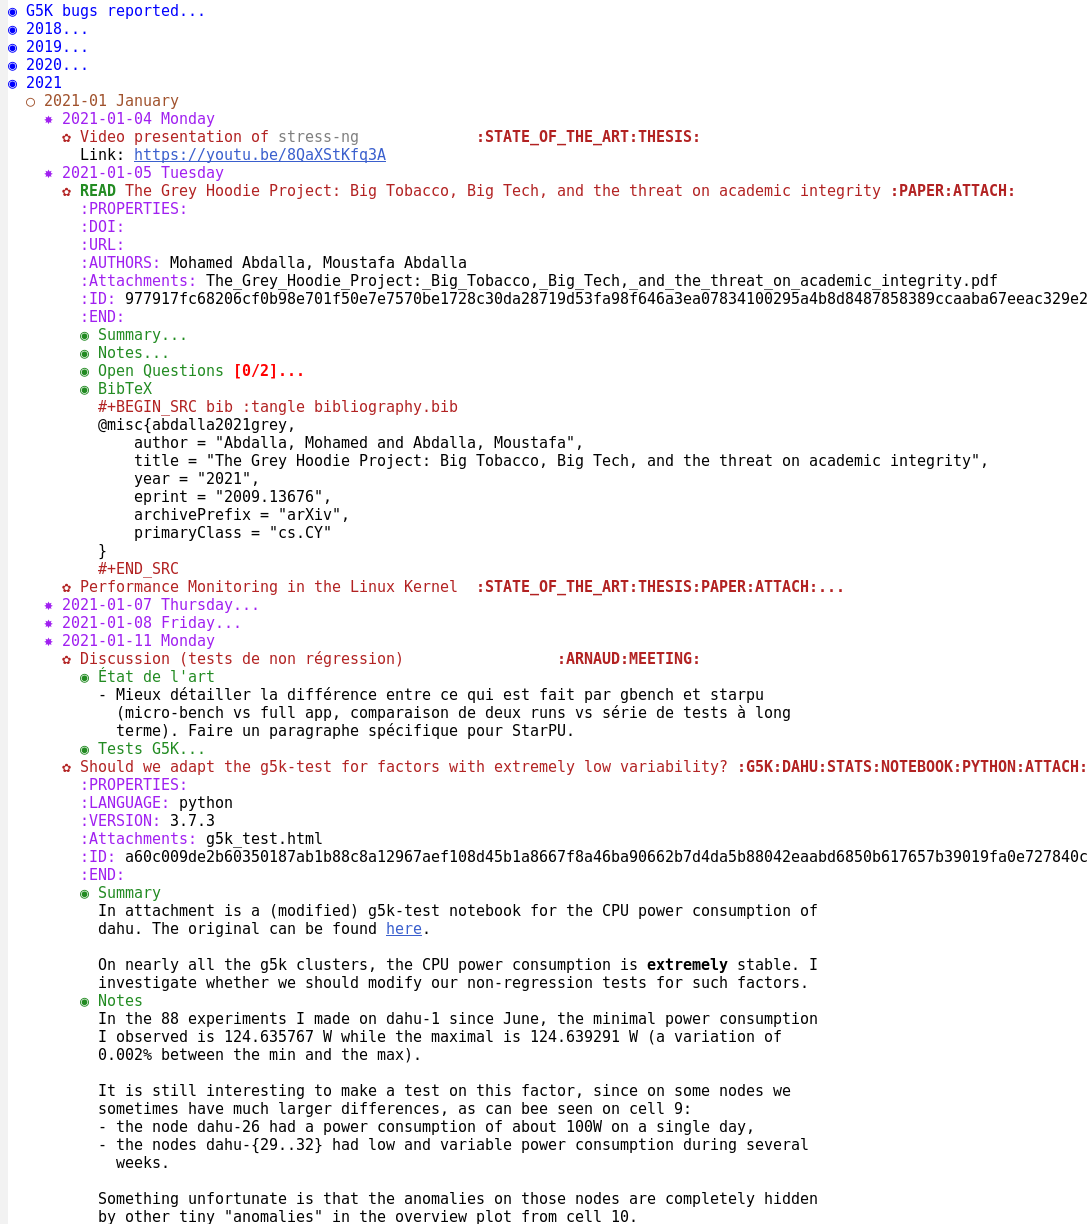
\includegraphics[width=\linewidth]{img/orgmode/journal_extract.png}}
        \caption{Screenshot of the laboratory journal used throughout this work.}%
        \label{fig:appendix:journal_extract}
    \end{figure}

    Such a rigorous method can appear as a waste of time, even overwhelming. We argue that despite the steep learning
    curve of org-mode, this time investment was worth it. We were able to come back to some early experiments several
    years later, understand precisely what these experiments were doing, and know with certitude the software versions
    that were used. Furthermore, we could also read the thought process we had at the time, the hypotheses we made that were later
    confirmed or rebutted. This is obviously of great help for reproducing these experiments or writing this thesis.

\chapter{List of software and data}
\label{chapter:zenodo}
    As this thesis was above all experimental, we implemented several programs to assist us in our work. Furthermore,
    the many experiments that we performed generated large amounts of data.  For the sake of reproducibility, both
    software and data are permanently archived on Zenodo. The full list is described in
    Table~\ref{tab:software_and_data}.

    \newcommand\tbelt[1]{\texttt{\textcolor{myblue}{#1}}}
    \begin{table}[htpb]
        \centering
        \caption{Software and data produced during this thesis.}
        \label{tab:software_and_data}
        \begin{tabular}{p{0.1\linewidth}p{0.8\linewidth}}
            \cite{peanut} &\tbelt{peanut} The experiment engine described in Section~\ref{sec:peanut}, written in
                Python. It allows to easily write scripts for deploying and running experiments, producing an archive
                with the experiment data and meta-data.\\
            \cite{cashew} &\tbelt{cashew} The Python library described in Section~\ref{sec:test:implementation} used for
                extracting the relevant data and meta-data from \texttt{peanut} archives, summarizing the data,
                computing non-regression tests on the aggregated data and generating the notebooks.\\
            \cite{org_attach} &\tbelt{org\_attach} A small Python script described in Appendix~\ref{chapter:orgmode} to
                add an entry in an Org-mode laboratory journal with an attachment (either a paper or a Jupyter
                notebook).\\
            \cite{calibration_analysis} &\tbelt{calibration\_analysis} Nearly all the experiment data produced during
                this thesis (\ie \texttt{peanut} archives) and the jupyter notebooks to analyze it. This includes MPI
                calibrations, \dgemm calibrations, real and simulated runs of HPL, etc.\\
            %&\tbelt{journal\_extract} \\
            \cite{g5k_test} &\tbelt{g5k\_test} The data and notebooks of the performance non-regression tests made on Grid'5000. This
                includes all the \texttt{peanut} archives, the HDF5 files containing the raw data, the CSV files
                containing the aggregated data and a full copy of the website presenting the test results.\\
            \cite{hpl_smpi} &\tbelt{hpl} The source code of High Performance Linpack, with the modifications we had to
                make for simulating its execution on top of SMPI.\\
            \cite{platform_calibration} &\tbelt{platform-calibration} The micro-benchmarks used to calibrate the models
                for the durations of \dgemm and MPI communications.\\
            \cite{pycewise} & \tbelt{pycewise} The Python library described in Section~\ref{sub:pycewise} for
                automatically computing piecewise linear regressions.\\
            \cite{ratatouille} & \tbelt{ratatouille} A Python script launched as a background process in experiments
                for monitoring system metrics such as the CPU temperature, core frequencies, CPU and DRAM power
                consumption.  These metrics are collected at a fixed pace (\eg every five seconds) and written in a CSV
                file.\\
        \end{tabular}
    \end{table}

    Additional material has also been archived once the defense had been carried out, the full list is described in
    Table~\ref{tab:additional_material}.
    \begin{table}[htpb]
        \centering
        \caption{Additional material archived after this thesis.}
        \label{tab:additional_material}
        \begin{tabular}{p{0.1\linewidth}p{0.8\linewidth}}
            \cite{defense_youtube} & \tbelt{defense} The video of this thesis defense, which was live-streamed on
                YouTube.\\
             & \tbelt{manuscript} The repository used for writing this manuscript and the slides of the defense. Besides
                the text and images, it also contains the code and a copy of the data used for generating the figures.\\
        \end{tabular}
    \end{table}

    Unfortunately, the laboratory journal described in Appendix~\ref{chapter:orgmode} could not be published, as it
    contained numerous copyrighted articles as well as confidential texts.

\chapter{Carbon footprint of this thesis}
\label{chapter:carbon}

    This thesis was written between November 2020 and March 2021, in the midst of the COVID-19 pandemic. At the time
    of the writing, more than two millions persons had already passed away and several millions will probably have long-term
    medical issues. Yet, this world disaster is arguably much less threatening than global warming. It is now established
    that the average temperature on Earth is increasing, mainly caused by anthropogenic emissions of greenhouse gases.
    It is difficult to estimate the damage that will be caused by global warming. The World Health Organization (WHO)
    writes that it is already causing \Num{150000} excess deaths per year~\cite{who_globalwarming_current} and that this
    figure is likely to rise to \Num{250000} per year between 2030 and 2050~\cite{who_globalwarming_future}, mainly
    caused by heat exposure, diarrhea, malaria and childhood undernutrition.  For the year 2018, according to the
    French government, the average carbon footprint of a French person is estimated to \NSI{11}{\tonne} of CO2eq.  This
    is more than five times larger than the yearly \NSI{2}{\tonne} target to limit the warming to
    \NSI{2}{\celsius}~\cite{co2_gouv}.

    For this reason, we felt it was important to compute the direct effect of this thesis on global warming. This
    chapter tries to estimate the greenhouse gases emission we generated, in carbon dioxide equivalent. We account for
    the two principal sources of CO2 emissions, \ie the business trips we made and the computing time we used on
    Grid'5000.  The goal is not to compute an exact figure, which would be extremely tedious, but rather to make a rough
    estimate and compare it to the \NSI{2}{\tonne} target.

    \subsection*{Business trips}%

        Several business trips done during this thesis required to take a plane. In the following, we will use the value
        of \NSI{195}{\gram/\kilo\meter} of CO2eq for long haul flight and \NSI{254}{\gram/\kilo\meter} for short haul
        flights~\cite{co2_flight}. We will neglect the emissions caused by the train travels, as this transportation
        mean is much less problematic (a French high speed train emits about \NSI{2}{\gram/\kilo\meter} for each
        passenger).
        \begin{itemize}
            \item On April 2017, I attended a Simgrid meeting in Bordeaux. I had to go by plane from Lyon
                (\NSI{435}{\kilo\meter}) as the train lines are very Paris-centered in France. This trip emitted about
                \NSI{0.2}{\tonne} of CO2eq.
            \item From October to December 2017, I visited Argonne National Laboratory in Chicago, USA. The outward
                flights went from Lyon to Frankfurt (\NSI{562}{\kilo\meter}) then to Chicago (\NSI{6967}{\kilo\meter}).
                The return flight went directly from Chicago to Paris (\NSI{6653}{\kilo\meter}).  In total, this trip has
                emitted approximately \NSI{2.8}{\tonne} of CO2eq.
            \item In November 2017, I attended the Supercomputing conference in Denver, USA. I went there with a direct
                flight from Chicago (\NSI{1475}{\kilo\meter}), emitting about \NSI{0.7}{\tonne} of CO2eq.
            \item In September 2019, I presented a paper at the Cluster conference, in Albuquerque, USA. The outward
                flights went from Paris to Los Angeles (\NSI{9085}{\kilo\meter}) then to Albuquerque
                (\NSI{1067}{\kilo\meter}). The return flights passed by Dallas (\NSI{586}{\kilo\meter}), then New York
                City (\NSI{2206}{\kilo\meter}) and finally Paris (\NSI{5837}{\kilo\meter}). This trip emitted
                approximately \NSI{3.9}{\tonne} of CO2eq.
        \end{itemize}
        Hence, the total amount of greenhouse gas emissions of this thesis due to airplane transportation is
        \NSI{7.6}{\tonne} of CO2eq.

    \subsection*{Computing time}%

        This thesis had a very important experimental component, it is therefore natural to expect a large amount of
        computing time usage. Figure~\ref{fig:appendix:node_hours} summarizes the cumulated computing time spent on
        Grid'5000 clusters during these years, grouped by usage type, for a total of \Num{2112014} core hours. The
        performance tests described in Chapter~\ref{chapter:experiment:tests} represent slightly more than half of this
        total time, which is very large. However, this should be contrasted by the consumption of the official Grid'5000
        tests: the \texttt{ajenkins} user, a bot responsible for periodically verifying the integrity of the platform,
        spent \Num{3272044} cores hours in the year 2020
        alone.\footnote{\url{https://intranet.grid5000.fr/stats/users.html}}

        Berthoud~\etal estimate the greenhouse gas emissions caused by GRICAD another French computing
        center~\cite{corehour_co2}. They tried to account for several parameters, including the electrical consumption
        of the hardware (computing nodes, storage nodes, network, cooling system), the manufacturing of this hardware,
        but also the emissions caused by the employees in charge of operating this computing center in their daily
        commute to work. They estimate that one hour of computation on one core is responsible for the emission of
        \NSI{5}{\gram} of CO2eq. The distribution of these emissions is depicted in
        Figure~\ref{fig:appendix:co2_per_hour}, slightly more than half of these \NSI{5}{\gram} is caused by the
        electrical consumption of the machine. It should be noted that French electricity is particularly low-carbon,
        meaning that this figure might be significantly larger in other countries that rely more on fuel and coal.

        \begin{figure}[tpb]
            \centering
            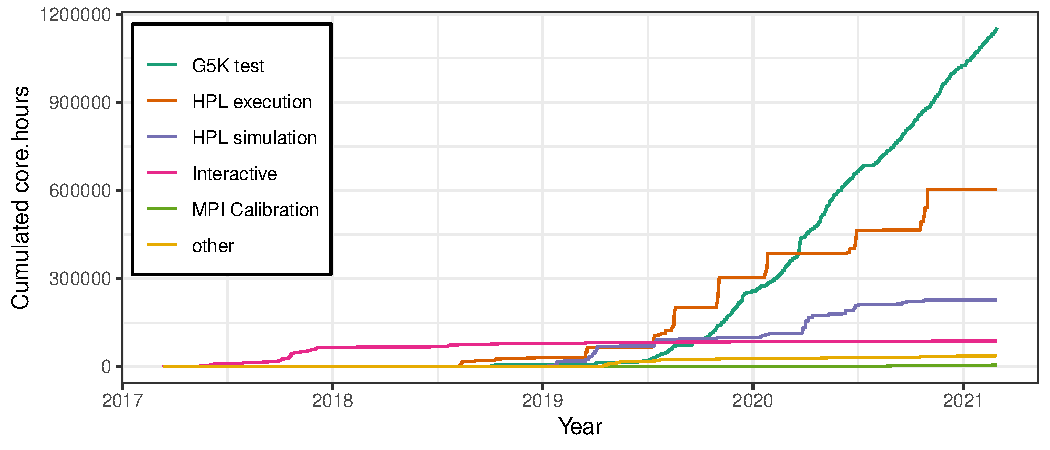
\includegraphics[width=\linewidth]{img/appendix/carbon/node_hours.pdf}
            \caption{Core hours used throughout this thesis for each experiment kind. In total, more than
            \Num{2112014} core hours have been used.}%
            \label{fig:appendix:node_hours}
        \end{figure}

        \begin{figure}[tpb]
            \centering
            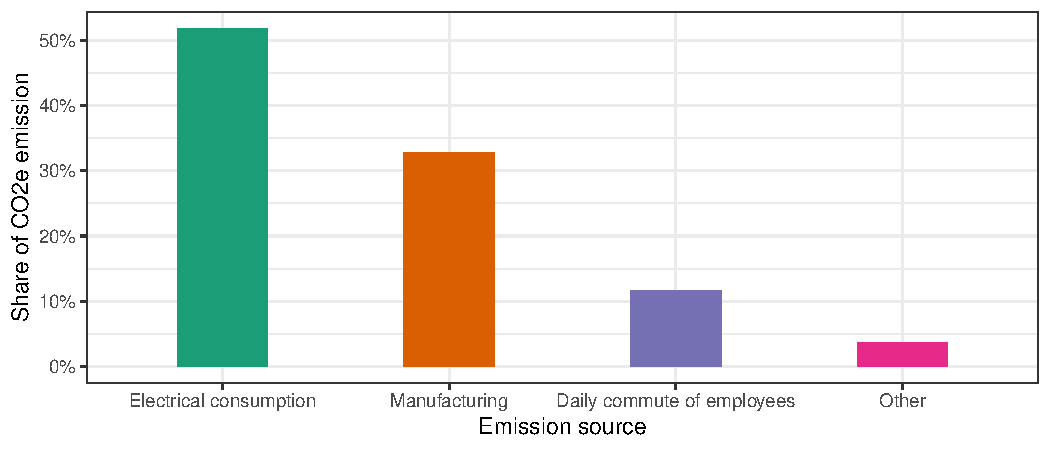
\includegraphics[width=\linewidth]{img/appendix/carbon/co2_per_hour.pdf}
            \caption{Source of greenhouse gases emission in a French scientific computing center, one core hour emits
            approximately \NSI{5}{\gram} of CO2eq~\cite{corehour_co2}.}%
            \label{fig:appendix:co2_per_hour}
        \end{figure}

        In the end, we estimate that the total amount of greenhouse gas emissions of this thesis due to computing is
        \NSI{10.6}{\tonne} of CO2eq.

        \subsection*{Conclusion}

            In this chapter, we tried to estimate the carbon footprint of this thesis. We do not claim to have an
            accurate figure to present (these back-of-the-envelope calculations are themselves based on rough
            approximations) but we should have the correct order of magnitude.

            We estimate that this thesis was responsible for the emission of \NSI{18.2}{\tonne} of CO2eq. This is
            significantly larger than the average yearly emission of a French person (\NSI{11}{\tonne} of CO2eq) and six
            times larger than the yearly target emission to limit the warming to \NSI{2}{\celsius} (\NSI{2}{\tonne} of
            CO2eq). Maybe counter-intuitively, this thesis emitted more greenhouse gases with computations than with
            airplane transportation, despite four transatlantic flights.
